\section{Unsupervised approach} \label{unsupervised_approach}

Here we present our first approach. It is inspired by the \acrfull{si} procedure performed by Microsoft to create the \acrfull{mag}, as outlined in a demo paper \cite{shen2018web}. We use the subjects they have discovered, as well as the hierarchy they extracted from the assignments. Details on their implementation can be found in section \ref{subject_indexing_mag}. Our goal is not to compare our results with Microsoft's, nor to fully reproduce their approach. Rather, our intention is to implement a fully unsupervised procedure, which doesn't depend on any external sources of data. We also require our implementation to be simple.

We have built a vocabulary based on the relevant documents of the repositories. At first, it contains all lemmatized tokens of the repositories. We then remove the tokens that appear in only one document, to reduce the size of the vocabulary. The details of the vocabulary construction can be found in section \ref{implementation_vocab}. We then train the embeddings of the vocabulary entries with the skip-gram model. The resulting vectors are used to vectorize documents and subjects, which are then compared in vector space regarding their similarity. In section \ref{implementation_skipgram}, we show the results of the training procedure and offer some examples.

We enrich the representation of documents by adding the representations of other documents that appear under the same venue, advisor and referee in the repositories. They handle similar topics, and therefore improve the representation of each other. Subjects, on the other hand, are enriched with text from their corresponding Wikipedia articles. We finally sort the words of each representation by frequency, removing duplicates. In section \ref{unsupervised_approach_representations}, we explain thoroughly how documents, subjects and venues are represented.

The representations of documents and subjects are then vectorized with the word embeddings. We compare them in vector space regarding the similarity, to find the subjects that should be assigned to each document. We have developed three methods to compute similarities, which we present in section \ref{unsupervised_approach_vectorization}, together with some examples that illustrate how they work. Adding together the word vectors of each representation seems to offer the best result. This will be properly tested in the evaluation (chapter \ref{eval}).

Finally, in section \ref{unsupervised_approach_conclusion}, we analyze the procedure, looking for decisive factors and possible improvements. The implementation is tedious, as it comprises many steps and details. Its accuracy can be increased by improving the vocabulary by discarding uninformative words and adding relevant phrases. Experimenting with other ways of representing texts, such as keeping duplicates, may also be beneficial.

\subsection{Building the vocabulary} \label{implementation_vocab}

The first step of the implementation is building the vocabulary. Words that are not included in it will be discarded when computing the vector representations for the documents, venues and subjects. Therefore, it is a very important step. It should include all words  that are relevant for the task of \acrshort{si}, i.e. the words that describe the topics each document handles.

The vocabulary is directly extracted from the corpus (the titles and abstracts of the documents). Only words that appear in the documents can be present in the vocabulary. There are several design choices that should be considered. We use SpaCy's small trained pipeline (called ``en\_core\_web\_sm'') for tokenization. The lemmatization is performed by the WordNet lemmatizer of NLTK, using the \acrfull{pos} tags computed by Flair's sequence tagger. The reasoning behind these choices are discussed in the following sections.

\subsubsection{Tokenizer}

Tokens are the semantic units that \acrfull{nlp} pipelines build upon. They are usually words, but depending on the task at hand, one can tokenize strings in different ways. For example, \textit{aren't} can be kept as a token or divided into two tokens, \textit{are} and \textit{n't}. This kind of decisions are made by the tokenizer, an algorithm that divides a given text into tokens. Tokenizers are usually based on simple heuristics.

We use the tokenizer from spaCy\footnote{\url{https://spacy.io/usage/linguistic-features\#how-tokenizer-works}}. It tokenizes words (which are surrounded by white spaces) by iteratively looking for prefixes and suffixes until a match is found with a regular expression that defines how a token should look like. Another reason why we pick this tokenizer is because it is included in Flair \cite{akbik2019flair}, an \acrshort{nlp} framework which we use later on to compute the \acrshort{pos} tags of each token.

\subsubsection{N-grams} \label{vocab_ngrams}

In some cases, words pose different meanings when combined with others. For example, ``ice cream'' has a particular meaning, and it should therefore be present in the vocabulary as a phrase. The words ``ice'' and ``cream'' pose different meanings when used independently. Such phrases also occur in the scientific jargon. For instance, ``machine learning'' refers to a field of computer science, something that cannot be deduced from its name. Still, the name describes well the purpose of the field (teaching machines how to learn). This is usually the case with scientific terms: they aim to describe their application as clearly as possible.

We built a vocabulary with n-grams of up to length four, to see its size and constituent entries. After filtering out the ones that appeared in only one document and those that appear in more than 1,000 documents, we found out that the n-grams weren't as informative as we expected. Many of them were just common sequences of words, such as ``this is a problem''. We talk about this vocabulary in detail in the appendix. We decided against including n-grams because the increase in quality was low compared with the increase in computational cost. 

\subsubsection{Vocabulary normalization}

The purpose of normalizing a vocabulary is to reduce its size by grouping words with similar meanings together. We will now introduce two normalization techniques that we have included in our procedure: case folding and lemmatization.

\paragraph{Case folding} \mbox{}

The most straight-forward way of reducing the size of the vocabulary is case folding. For example, the word ``here'' may be capitalized because it is at the beginning of the sentence and would thus appear as another entry in the vocabulary. Writing all words in lower case eliminates this duplicity issue.

Case folding is not suitable for tasks where proper nouns should be identified. For example, the word ``frank'' has a different meaning than the name ``Frank''. This issue is not relevant for our task, as we are mainly interested in scientific words that have unique meanings. Therefore, we perform case folding on all words before adding them to the vocabulary.

\paragraph{Lemmatization} \mbox{}

Lemmatization consists of replacing words by their semantic roots. It makes the model more general by removing verb conjugations, plural cases and other variations of words that ultimately have the same meaning. This technique may also reduce the precision of the model. For instance, words with different meanings, such as ``bank`` and ``banking'', are reduced to the same lemma even if the meaning of the word ``bank'' is context-dependent. Such situations are a priori not dangerous for our task, as scientific words usually have concise meanings.

Stemming is a similar approach, in which prefixes and suffixes are removed. For example, the stem of the word ``house'' is ``hous'' and its lemma is ``house''. Lemmatization is more accurate because it takes into account the meaning of the word \cite{hapke2019natural}. A good example of this is ``better'', whose lemma is ``good'' while its stem is ``bet'', which has a completely different meaning. Because of this, lemmatizers are suitable for more applications, and ours is no exception.

We use the WordNet lemmatizer of the NLTK package in our pipeline. WordNet \cite{fellbaum2010wordnet} is a lexical database that is publicly available and offers lemmatization. NLTK provides an interface to this lemmatizer. The accuracy of the lemmatization improves when the \acrfull{pos} tag of the word that should be lemmatized is also provided. We do so using the fast universal \acrshort{pos} tagger from Flair \cite{akbik2019flair}, called ``upos-fast''. The model, which combines Flair's contextual word embeddings \cite{akbik2018contextual} with a LSTM-CRF model, is trained on the data set of the CoNLL's shared task of 2018 \cite{zeman2018conll}, which comprises words in 12 languages. The resulting tagger has an F1-score of 98.47\footnote{As seen here (accessed on 06.07.2021): \url{https://github.com/flairNLP/flair/blob/master/resources/docs/TUTORIAL_2_TAGGING.md}} on the Ontonotes data set, only behind its larger version, called ``upos''. The difference between them is too small (0.13) to account for the large difference in performance. Using the faster model speeds up the procedure by around 500 \%.

\subsubsection{Vocabulary filtering} \label{vocab_filtering}

Once the vocabulary has been created, we remove the entries that occur in only one document, as their meanings may be too specific to relate documents to one another. Entries that are either stop words\footnote{For this purpose, we use NLTK's list of English stop words, which comprises 179 words as of 07/07/2021.} or punctuation signs are also discarded. Symbols such as Greek letters are kept, as they refer to certain concepts in fields like Physics or Mathematics.

At first, we discarded entries that occur in more than 1,000 documents, which reduced the size of the vocabulary to 49,651 entries. However, this also resulted in 7,188 documents not having any words that were in the vocabulary, meaning that they could not be vectorized. Given that there are only 488 vocabulary entries that occur in more than 1,000 documents, we decided to keep them. This greatly improves the coverage: now only 85 documents cannot be represented.

\subsubsection{Resulting vocabulary} \label{vocab_results}

In our corpus, there are 125,575 distinct tokens. 75,436 of them appear in only one document and are discarded. Thus, the final vocabulary comprises 50,139 entries. With this vocabulary, only 85 documents cannot be represented, i.e. none of the words of their titles and abstracts appear on the vocabulary. Keep in mind that 51 of those documents didn't have any texts to begin with, as stated in section \ref{repo_analysis_data}.

In figure \ref{fig:bow_data}, the number of tokens of the documents that are included in the vocabulary is displayed. As mentioned before, 85 documents don't have any of their tokens in the vocabulary. 110 have just one. On the other end of the spectrum, 24,819 documents have nine or more tokens in the vocabulary. This accounts for 84 \% of all documents. Vocabulary entries appear on average on 27.1 documents. Figure \ref{fig:vocab_1grams} shows in how many documents each entry of the vocabulary occurs, grouped in bins. 46,776 entries (94 \%) appear in 100 documents or fewer. 15,250 entries (31 \%) appear in only two documents.

\begin{figure}
    \centering
    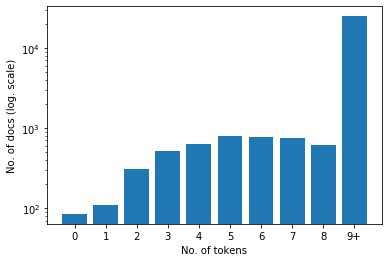
\includegraphics[width=.7\textwidth]{figures/unsupervised_approach/bow_data.png}
    \caption{Distribution of the documents depending on the number of their tokens that are included in the vocabulary.}
    \label{fig:bow_data}
\end{figure}

\begin{figure}
    \centering
    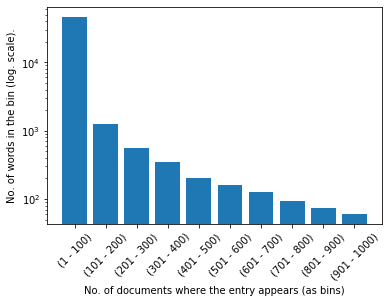
\includegraphics[width=.7\textwidth]{figures/vocab/vocab_1grams.png}
    \caption{Distribution of the vocabulary entries depending on the no. of documents they are included in.}
    \label{fig:vocab_1grams}
\end{figure}
\subsection{Embedding model} \label{implementation_skipgram}

To transform text into vectors, we first embed words into vector space. We could do so randomly, but this wouldn't take into account the semantic information of the words. To preserve this information, we use skip-gram \cite{mikolov2013distributed}, a word embedding model. This model was also used by \acrshort{mag} in their procedure. We already gave an overview of its design in section \ref{mag_skipgram}. In this section, we will look at how we trained the model and some examples of the resulting embeddings.

We train 100-dimensional word vectors, which we initialize with values sampled from the uniform distribution bounded by -1 and 1. The word vectors of \acrshort{mag} comprise 250 dimensions. We have decided to use fewer dimensions given that our vocabulary is much smaller: it includes around 50,000 entries, whereas \acrshort{mag}'s vocabulary has than 2 million.

We trained the model for 8 epochs. Surprisingly, it reached its best epoch loss already in the second iteration. The model optimized the embeddings quickly during the first epoch, starting with a batch loss of $30$ and ending with an average epoch loss of $4.9$. Figure \ref{fig:loss_avgs} shows the avg. loss of each epoch. Figure \ref{fig:loss_avgs_range} also shows the avg. loss, but with bars illustrating the range of the batch losses throughout the epoch.

\begin{figure}
  \begin{subfigure}[t]{0.5\textwidth}
    \centering
    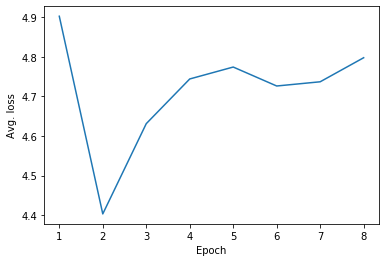
\includegraphics[width=\textwidth]{figures/unsupervised_approach/loss_avgs.png}
    \caption{Avg. training loss of each epoch.}
    \label{fig:loss_avgs}
  \end{subfigure}
  \hfill
  \begin{subfigure}[t]{0.5\textwidth}
    \centering
    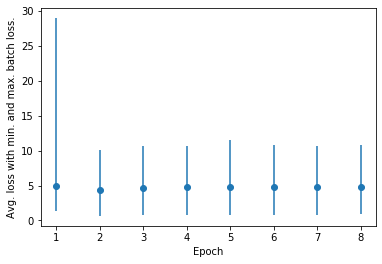
\includegraphics[width=\textwidth]{figures/unsupervised_approach/loss_avgs_range.png}
    \caption{The dots refer to the avg. epoch loss, while the extrema of the line refer to the min. and max. batch loss of that epoch.}
    \label{fig:loss_avgs_range}
  \end{subfigure}
  \caption{Plots of the training loss of the skip-gram model.}
\end{figure}


\subsubsection{Resulting embeddings}

We have computed the cosine distance between certain words to serve as an example. The cosine distance is also the metric we use to compare subjects and documents. The results can be found in table \ref{tab:embeddings_examples}. We have chosen three pairs of words, each of a different field. `polymer'' and ``monomer'' belong to the realm of chemistry; ``machine'' and ``learning'' usually refer to a family of algorithms; ``magnetic'' and ``resonance'' refer to a medical procedure. The chemistry pair is fed to the skip-gram model 96 times during training; the computer science pair, 1357 times and the medicine pair, 961 times.

Given that the cosine distance is symmetric, we only show one half of the table. Also, the distance of a vector to itself is zero. The table shows that the pairs of words of each field are closer to each other than to the other words. The distance between ``polymer'' and ``monomer'' is the largest of the three, which makes sense, as the model receives this pair of words hundreds of times less than the two others. The smallest distance between words that do not belong to the same field is between the words ``magnetic'' and ''polymer''. This distance is 34 \% larger than the distance between ``monomer'' and ``polymer''. Thus, the word vectors accurately differentiate between words that belong to the same field and those that don't.

As a further example of the semantic expressiveness of the embeddings, we can look at the word ``program'', although it belongs to the same field as the computer science pair, it is not as closely related to them. In fact, it appears 27 times as an input to the model with either of the words ``machine'' and ``learning''. However, this is more often as for the pairs of chemistry and medicine, with which it appears as input 26 and 3 times, respectively. The model was able to identify that ``program'' should be closer to the computer science pair, even if it appeared only one time less with the chemistry pair. Its cosine distance to ``machine'' and ``learning'' are 0.77 and 0.72, respectively. On the other hand, its cosine distance to the rest of the words is above 1.

\begin{table}[]
    \centering
    \begin{tabular}{c|c c c c c c}
       $dist(x,y)$ & monomer & polymer & machine & learning & magnetic  \\
       \hline
       resonance & 0.96 & 0.91 & 0.95 & 0.95 & \textbf{0.21} & \\
       magnetic & 0.88 & 0.82 & 0.98 & 0.98 & & \\
       learning & 1.08 & 1.19 & \textbf{0.41} & & & \\
       machine & 1.02 & 0.95 & & & & \\
       polymer & \textbf{0.54} & & & & & \\
    \end{tabular}
    \caption{Cosine distances between the vectors of certain words. The distances of words of the same field are highlighted in bold.}
    \label{tab:embeddings_examples}
\end{table}
\subsection{Vector representations} \label{unsupervised_approach_representations}

In this section, we talk about the vector representations of the three different elements of our corpus (documents, venues and subjects). This procedure is an adaptation of \acrshort{mag}'s approach \cite{shen2018web} to our scenario. An important difference between our setting and that of \acrshort{mag} is that ours includes theses, which are not published in any venue.

In the following three sections we will look at the information used to represent venues, documents and subjects. Each element has both a \acrfull{srt} and an \acrfull{ert}. The \acrshort{srt} consists of basic information of the element, whereas the extended one comprises information of associated elements, which are used to enrich the representation of each element.

\subsubsection{Venues}

Venues are journals, conferences and other organizations where researchers can publish their work. They usually accept publications regarding a certain field, such as the \textit{Journal of Clinical Medicine}, which publishes medical work. Some are even more specific, such as the \textit{International Conference on Dublin Core and Metadata Applications}, which only includes publications that have to do with metadata, an area of computer science. Others are more interdisciplinary, including publications of different fields. An example of such a venue is the \textit{Journal of Chemical Physics}, which is a subdiscipline of both Chemistry and Physics. There are venues that are even more broad, such as the famous \textit{Nature}, which comprises all natural sciences and technology.

Regardless of their scope, venues can be useful to identify what topics their publications revolve around. Therefore, the representations of venues are used in the representations of documents. Specifically, their representations are added, with the venue's representation being weighted down. The venues present in the repositories were already analyzed in section \ref{repo_analysis_venues}. Given that there are many types of venues, they appear under various names in the repositories, such as \textit{Journal title} or \textit{Proceedings}. How venues are stored also differs between repositories.

An important difference between our use case and \acrshort{mag}'s, is that we also consider theses, which are not published in any venue. We argue that advisors and referees have a similar role for theses as venues have for publications. We therefore use them as a replacement for venues when considering theses. We then look at how \acrshort{mag} computes the \acrshort{ert}s of venues, and how we do so in our use case. In the end, venues are represented by a sample of the documents they are assigned to, whose representations are concatenated.

\paragraph{Alternative venues for theses} \mbox{} \label{unsupervised_approach_venues_theses}

Given that 36 \% of our documents are theses and thus were not published anywhere, we require a workaround that allows for theses to also be grouped by the topics they handle. If we didn't find an alternative, the representations of theses would be considerably less precise than those of publications, which would hamper the quality of the \acrshort{si}. Just as venues publish research work that handles the topics they focus on, referees and advisors of theses only do so when the topics handled by the student aligns with their fields of expertise. They are therefore good indicators of the semantic content of a thesis.

As discussed in section \ref{repo_analysis_contributors}, theses of edoc and refubium almost always have at least one referee (only 1 \% and 5 \% of the theses don't have one, respectively). On the other hand, 19 \% of the theses of depositonce are missing a referee. The missing referees in depositonce are luckily replaced by advisors. Depositonce is the only repository where advisors appear often. Only 4 \% of the theses there don't have one. Edoc and refubium have almost no advisors.

Given the differences among the repositories, both referees and advisors have to be considered as an alternative for venues when grouping theses. When doing so, only 5 documents of depositonce (0.07 \%) don't have an expert (i.e. neither an advisor nor a referee). 30 documents of edoc (0.4 \%) are also missing an expert, as well as 662 documents of refubium (5 \%). These and other facts are shown in table \ref{tab:experts}, including that, on average, theses feature more than two experts. This may help identify the topics of theses that are multidisciplinary, i.e. whose subjects belong to several fields.

\begin{table}[]
    \centering
    \begin{tabular}{|c|c|c|c|c|}
    \hline
         \thead{Repository} & \thead{No. of \\ experts} & \thead{No. of distinct  \\ experts} & \thead{Avg. no. \\ of experts \\ per thesis} & \thead{No. of theses \\ without \\ an expert} \\
         \hline
         depositonce & 8,383 & 2,338 & 2.6 & 5 (0.07 \%) \\
         \hline
         edoc & 7,308 & 3,395 & 2.8 & 30 (0.4 \%) \\
         \hline
         refubium & 9,133 & 4,863 & 2.2 & 662 (5 \%) \\
         \hline
    \end{tabular}
    \caption{Facts regarding the experts of theses.}
    \label{tab:experts}
\end{table}

\paragraph{Simple representation} \mbox{}

\acrshort{mag} uses the name of the publishing venue as its \acrshort{srt} \cite{shen2018web}. For referees and advisors, we could use the name of the person as its \acrshort{srt}. However, the names of professors have no relationship with their fields of expertise, and therefore would not provide any information about the topics they work on. We therefore discard the names of venues altogether, for the sake of simplicity.

\paragraph{Extended representation} \mbox{}

\begin{figure}
    \centering
    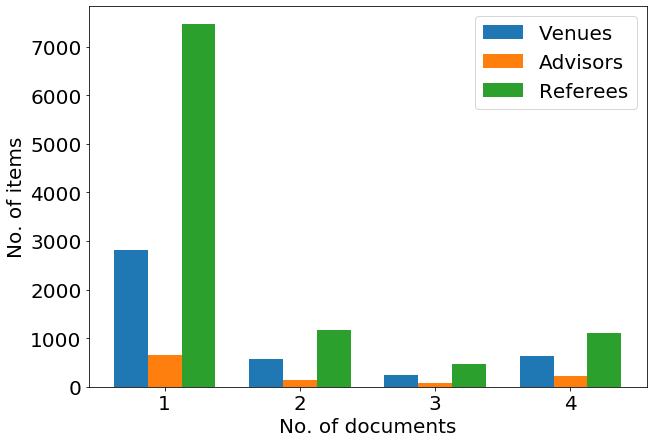
\includegraphics[width=.7\textwidth]{figures/unsupervised_approach/ert_counts.png}
    \caption{No. of documents included in the creation of the ERT of venues, referees and advisors.}
    \label{fig:ert_counts}
\end{figure}

The \acrshort{ert} of a venue is formed by concatenating the \acrshort{srt}s of a sample of its publications. The authors of \acrshort{mag} don't specify how many publications they use for the \acrshort{ert} of each venue. Given that our venues have on average 4.2 publications assigned to them, we pick 4 as the maximum sample size. Venues with less than four documents will take as many documents as there are available to compute their \acrshort{ert}. We do the same for advisors and referees. Those that have more than four documents available are assigned the four longest documents in terms of the number of tokens that are present in the vocabulary, instead of randomly sampling four documents. In this way, we improve their representations by ensuring they comprise as many tokens as possible.

Figure \ref{fig:ert_counts} shows how many documents are used to represent each item (venue, referee or advisor). Most of the items only include one document in their representations. This is the case for 66 \% of the venues, 59 \% of the advisors and 73 \% of the referees. This fact will be important when evaluating the accuracy of our vector representation for the items. Items that include more documents are expected to have more accurate vector representations.

There are six venues and thirteen referees that cannot be represented. Even if they have documents assigned to them, these do not include any tokens that are present in the vocabulary. There are also several more that have only a few tokens on average, as can be seen in figure \ref{fig:bow_venues}. On the other hand, there are only three advisors with less than nine tokens on average. These averages refer to the avg. amount of tokens of their constituent documents, i.e. those that were picked for their \acrshort{ert}.

\begin{figure}
    \centering
    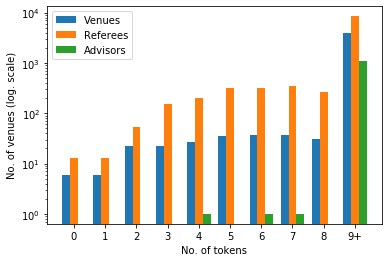
\includegraphics[width=.7\textwidth]{figures/unsupervised_approach/bow_venues.png}
    \caption{Avg. number of tokens of venues, referees and advisors.}
    \label{fig:bow_venues}
\end{figure}

\subsubsection{Documents}

Documents are the publications and theses of the repositories that are written in English. The \acrshort{srt} of a document comprises its title and abstract, and the \acrshort{ert} results from concatenating the \acrshort{ert} of its venue. In this section, we will look at both representations, comparing our implementation with that of \acrshort{mag}. There are some challenges that arise from the small size of our dataset. For instance, the extracted references often pointed to papers outside our dataset, being thus of no use to relate documents to one another.

\paragraph{Simple representation} \mbox{}

Creating the \acrshort{srt} of the documents is straight forward. We can extract the title and the abstract of a document through the OAI-PMH interface of each repository. \acrshort{mag} also uses the keywords, but these are not available in the metadata of the papers. We therefore only use the title and the abstract to represent each document. We cannot use the subjects assigned by the users that uploaded the documents because these will be used to evaluate the performance of our model.

We discard using the full texts of the documents because doing so would complicate the encoding task. Only the most important aspects covered by the paper are included in the abstract, which are the ones we want to consider. Using the full texts could potentially reduce the quality of the encodings, as they cover topics that are not central to the ``aboutness'' of the paper, such as the related work. Furthermore, extracting the texts from the PDFs is time-consuming and computationally expensive.

After processing the texts and removing the tokens that are not included in the vocabulary, documents have on average 37 tokens. 85 documents don't have any, and over 84 \% of them have nine or more tokens. These and some other facts, along with figure \ref{fig:bow_data}, were already discussed in section \ref{vocab_results}, as they were used to determine the size of the vocabulary.

\paragraph{Reference and citation extraction} \mbox{} \label{unsupervised_approach_references}

A reference used by a document $A$ is another document $B$ which the document $A$ uses to lay the foundation of their work. It gives the reader an understanding of the scope of their work, as well as the fields involved. Document $B$ is then cited by document $A$, i.e. citations can be understood as the inverse relations of references: if document $B$ is a reference of document $A$, document $A$ is a citation of document $B$.

To extract the references from the papers, we use a package called \textit{refextract}\footnote{\url{https://github.com/inspirehep/refextract}}. It returns the references it finds in a given text as a dictionary, which includes the title, authors, journal title and other data about each of the referenced papers. Refextract uses regular expressions to identify the elements of the reference, as well as mappings for special cases. It was developed to be used for scientific papers of \textit{High-Energy Physics}\footnote{\url{https://www.energy.gov/science/hep/high-energy-physics}}, an American laboratory. This means that the special cases included in the knowledge bases focus on this specific set of papers. Therefore, we expect the accuracy to be worse in our heterogeneous dataset, which comprises papers written in various formats as well as theses.
 
Using this package, together with a Python port to the Apache Tika library\footnote{\url{https://github.com/chrismattmann/tika-python}} to parse the text from the PDF files, we successfully extracted the references of 29,329 documents. Only 5 documents of depositonce and 14 of refubium didn't have any references. In edoc there are 50 files where no references could be extracted. These documents either did not have any files, the file did not include references, or the format of the references could not be identified.

The documents for which we could extract references, include on average 157 references. This number is so large because of the theses, which on average comprise 246 references. Publications include on average 105 references. This number is so large because of refubium, whose documents include on average 121 references. Edoc and depositonce include 85 and 91 references on average, respectively. Unfortunately, most of these references point to documents outside the repositories. Only 328 documents (1.2 \% of all the documents) refer to other documents in the repositories. They do so an average of six times. The remaining 29,001 documents (99 \% of all documents) cannot be related through their lists of references.

\paragraph{Extended representation} \mbox{}

In \acrshort{mag}, the \acrshort{ert} of a document comprises three different aspects (references, citations and venues). As was just mentioned, the size of our dataset is too small to profit from relations among papers through their lists of references. Therefore, we only use the \acrshort{ert} of its associated venues, referees and advisors. These are added to the \acrshort{srt} after being multiplied with a weighting factor $w$. Here is the equation for computing the \acrshort{ert} of documents:

$$ h_e^d = h_s^d + w \cdot \frac{1}{n} \sum_V h_e^V $$

$h_s^d$ refers to the \acrshort{srt} of a document; $h_e^V$ refers to any venue, advisor or referee that is related to the document. The creators of \acrshort{mag} don't disclose how they weighted venues in the paper. Therefore, we decided to choose $0.7$ as the weight parameter. Our choice is probably higher than the one used in \acrshort{mag}. This makes sense as we have less data available to represent documents.

Once the representations of documents are enriched with the representations of their venues, only 33 documents remain without tokens, out of the 85 that were empty before. The number of tokens per document is illustrated in figure \ref{fig:doc_representations}, which can be compared to figure \ref{fig:bow_data}, where the same data is shown but without including venues. On average, document representations comprise 324 tokens, including tokens of 1.5 venues. 20,399 documents include only one venue, whereas 7,430 documents include either two or three venues. Almost 98 \% of the documents have more than eight tokens in their \acrshort{ert}.

\begin{figure}
    \centering
    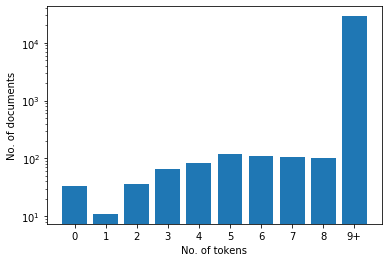
\includegraphics[width=.7\textwidth]{figures/unsupervised_approach/doc_representations.png}
    \caption{Number of tokens in the extended representation of the documents.}
    \label{fig:doc_representations}
\end{figure}

\subsubsection{Subjects}

Subjects are the concepts we use to describe the content of the documents. Each document is assigned a variable number of subjects, which together define what the document is about. We already discussed how subjects were retrieved from OpenAlex in section \ref{problem_scope_subjects}. The resulting set comprises 2,157 subjects, evenly distributed among the 19 fields.

Here, we explain what information we use to describe the subjects. Microsoft performed manual steps to create the \acrshort{ert} of the subjects that we are unable to emulate. Therefore, subjects only comprise a \acrshort{srt}, which is their Wikipedia article. This is the only external information we use throughout this approach, as we have not found any other way to represent subjects.

\paragraph{Simple representation} \mbox{}

Each \acrshort{mag} subject is associated to a Wikidata page, from which we can extract the Wikipedia link. We parse the HTML tree of the Wikipedia pages with the \textit{lxml} package\footnote{See \url{https://github.com/lxml/lxml}}, which allows us to navigate the tree with XPath expressions. We use them to avoid retrieving the texts of quotes, tables, or images, which sometimes appear before the content of the page. Once we arrive at the content, we retrieve paragraphs until we have gathered at least 500 characters.

If there is no link to an English Wikipedia entry, we use the Wikidata description as the \acrshort{srt}. This is the case for only three subjects: \textit{Discretization}, \textit{Statute} and \textit{Interim}. The \acrshort{srt}s of these subjects comprise 71, 40 and 33 characters, respectively. All other subjects have \acrshort{srt}s with more than 500 characters.

On average, the \acrshort{srt}s of the subjects comprise 752 characters. Regarding tokens that are present in the vocabulary, the Wikipedia articles have on average 30 tokens. Only four subjects have less than nine tokens: the three for which no Wikipedia page was found and \textit{Athletes}, whose Wikipedia page really consists of just one sentence.

\paragraph{Extended representation} \mbox{}

The research group of Microsoft manually assigned subjects to venues and used the \acrshort{ert}s of a sample of venues as the \acrshort{ert} of the subject. Doing so is a lot of work, which is out of reach for this thesis, as we don't have the manpower of Microsoft. We therefore only use the Wikipedia articles to represent the subjects.

\subsection{Vectorizing the representations} \label{unsupervised_approach_vectorization}

Once all the appropriate texts have been retrieved to represent each document and subject, the next step is to vectorize the representations. Before replacing words by their corresponding vectors, we order the words of each document and subject by frequency, so the most frequent ones are at the front. The words of the venues, advisors and referees are added in a weighted manner to their associated documents before the sorting occurs.

We then present three different methods in which we compute cosine distances, which are based on concatenation, averaging and addition. We will offer some examples afterwards, which show that summing the vectors yields the most interpretable results. The proper experiments with them are presented in chapter \ref{eval}.

\subsubsection{Item representation} \label{unsupervised_approach_our_representation}

Before replacing the words of a text with vectors, we count how often each word occurs and sort them by frequency. This is important because when computing cosine distances we may remove some vectors of a representation, so the representations of documents and subjects match in size.

Documents are represented both by their own words and those of its associated venues, but the latter are weighted down. Here we first join the counts of the document's representation and the weighted counts of the venue's representation before sorting them. Once the words of a representation are sorted, we replace them with vectors. The length of these representations was already presented in section \ref{unsupervised_approach_representations}.

\subsubsection{Computing cosine distances}

We have considered three ways of computing cosine distances. Given the word vectors of a document and a subject, we can:

\begin{enumerate}
    \item compute one cosine distance where the word vectors are concatenated,
    \item compute the cosine distance between each pair of words (one from the document and one from the subject), and then average over the resulting distances or
    \item compute one cosine distance where the word vectors are summed.
\end{enumerate}

Concatenating the vectors is the easiest way to proceed. All vectors representing each document and subject are gathered into one, making the computation of the cosine distance straight forward. This is the method used in the \acrshort{mag}. Averaging over the word vectors differs from the other two in that word vectors are compared independently. Here it is therefore important that words are ordered by frequency, so the most relevant words of a document are compared with the relevant ones of the subject.

The possibility of adding the word vectors together arises from the linear relationships between the skip-gram embeddings \cite{mikolov2013distributed}. The authors argue that this property can be explained with the training objective, where adding word vectors is equivalent to multiplying their context distributions. Thus, words that often appear together can be associated by addition.

\subsection{Results} \label{unsupervised_approach_results}

Once we have the vector representations of documents and subjects, we can compute the cosine similarity between them to determine how similar they are regarding their semantic content. Due to the hierarchical nature of the subjects, we first compute the similarities of every document with the subjects of the first level, what we call fields, and then compute the similarities for the descendants of the five most similar fields for each subject. We then store the 50 most similar subjects.

However, we first have to choose how to compute the similarities between documents and subjects. The proper experiments with the methods are presented in chapter \ref{eval}. Here, we discuss some examples and perform a qualitative assessment of the three methods. We only consider fields to not compute so many similarities, as they are expensive.

\subsubsection{Word vector combination} \label{unsupervised_approach_results_combination}

\begin{figure}
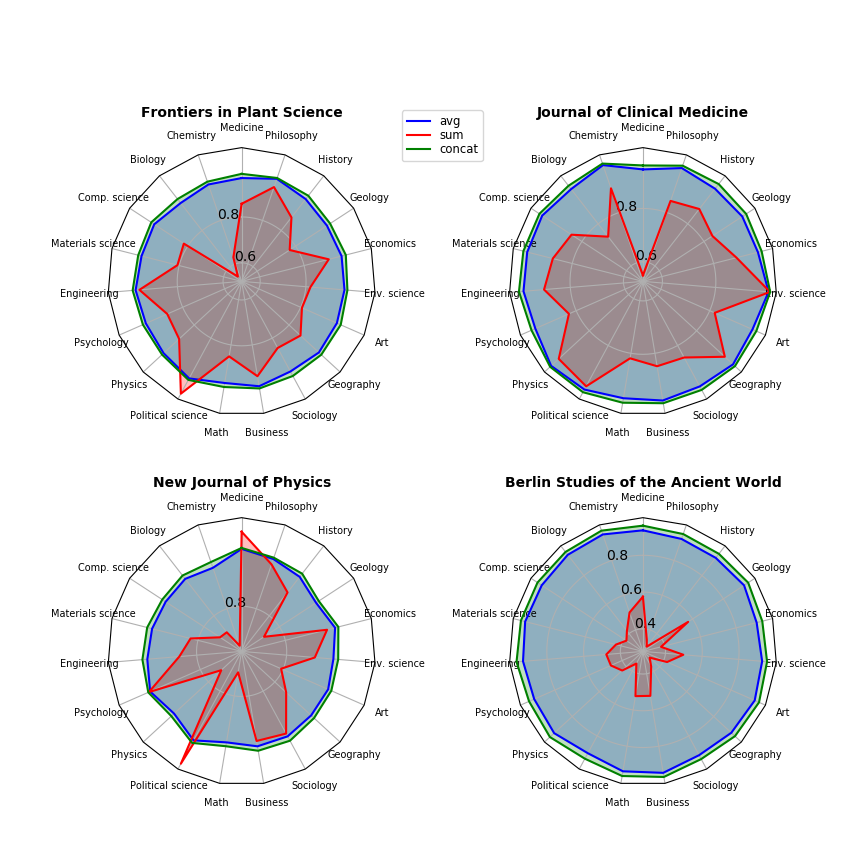
\includegraphics[width=\textwidth]{figures/unsupervised_approach/results/radar charts.png}
  \caption{Distances between venues and fields, for the three distance metrics.}
  \label{fig:combination_distance}
\end{figure}

In figure \ref{fig:combination_distance}, we show the results of the three methods for four venues, each belonging to a different field. The distances shown are the average distances of the documents that belong to each of the venues. In the upper left corner, the average distances of the documents that were published in \textit{Frontiers in Plant Science} are shown, which belongs to the field of \textit{Biology}. All three methods successfully identified the correct field on average.

The \textit{sum} method has the most expressive results. It assigns the documents \textit{Chemistry} in second place, and the distance between \textit{Biology} and \textit{Chemistry} exceeds $0.1$. On the other two methods, all three top options differ by around $0.01$. In fact, in the figures, one can see that the average distances of the concatenation and averaging methods are always around $0.95$. The difference between them occurs at a much lower scale. This shouldn't be a problem, as the distances can be rescaled afterwards.

All three methods also identified correctly the field of the venue \textit{Journal of Clinical Medicine}, shown in the upper right corner of figure \ref{fig:combination_distance}. Even for the averaging and concatenation methods, it is clear to see the smaller distance for the \textit{Medicine} field.

In the lower left corner, the average distances for the publications of \textit{New journal of Physics} are shown. None of the three methods places \textit{Physics} among their top three fields. The averaging and sum methods guess \textit{Chemistry} as the top field, whereas the concatenation method guesses \textit{Geology}. Physics is expected to be harder to guess because of its ubiquitous impact. It is closely related to other fields, mainly because it can be applied to any natural science.

The average distances between the fields and the documents published in \textit{Berlin Studies of the Ancient World}, which encompasses research in the fields of \textit{History} and \textit{Philosophy}, are shown in the lower left corner. The sum method was the only one to include both fields in their top three guesses, with \textit{Geography} between them. The other two methods guessed \textit{Political Science}, \textit{Economics} and \textit{Sociology}. Although similar, these were not the correct fields.
\subsection{Conclusion} \label{supervised_approach_conclusion}

We conclude this chapter by discussing the complexity of the implementation and some aspects of the model that may be improved to increase the performance of the model. The implementation of the models, as well as gathering the training data, is easy to develop. On the other hand, processing the training data training the models is computationally expensive.

We propose several improvements, mostly regarding the fact that the subject assignments are performed by an algorithm and not by a human. This means that its assignment noise could be modeled more easily, as the algorithms operates in a deterministic manner, whereas humans are not so consistent. Also, the assignment algorithm outputs confidence scores, which could also be used to improve the training procedure.

\subsubsection{Implementation}

The supervised approach was easy to implement. Gathering the training data didn't pose any difficulties because of the \acrshort{api} provided by OpenAlex. We vectorized the data in the same way we vectorized the documents of the repositories. Implementing the model also didn't pose any major challenges, as we used the architecture of related work \cite{gargiulo2019deep}. The further two papers we have implemented extended this initial model, both by modifying the loss function and one with an additional layer. Thus, the implementation time was much shorter than that of the unsupervised approach, which included numerous steps. On the other hand, this approach required training many models, which is computationally expensive. Processing the training data is also expensive.

\subsubsection{Room for improvement}

The hit rate of this approach can be easily improved by gathering more training data. Also, there are many techniques regarding the design and training of neural networks that may be experimented with, such as introducing batch or layer normalization \cite{ba2016layer}. Furthermore, there are two aspects from our use case that we have not considered:

\begin{enumerate}
    \item \textbf{Noise distribution}: model noise can be better modeled than human noise, because it is deterministic. Doing so would increase the performance of the model.
    \item \textbf{Confidence scores}: models output confidence scores for the subject assignments, which could be included in the training procedure, e.g. as a replacement of binary labels.
\end{enumerate}

Both aspects derive from the nature of our training dataset, which was created by an algorithm rather than by humans. Addressing these two points could lead to further improvements in the performance of the model. Label noise is a common topic in the literature, as it is present in all datasets labeled by humans because of their inconsistency (\cite{morris2010individual}, \cite{medelyan2008domain}). Deep networks must handle noise appropriately because, if not, they may overfit on the corrupted labels \cite{chen2019understanding}. There are three ways of handling noise \cite{karimi2020deep}: through the selection of the model and the loss function, by cleaning the data, or by developing a model that models label noise.

We have performed several data cleaning tasks, such as checking the language of the texts (see section \ref{repo_analysis_data}). Furthermore, the \acrlong{asl} models label noise better than \acrlong{bce}, as noise is not symmetric across positive and negative samples, given that positive ones are sparse \cite{zhao2021evaluating}. Still, modeling label noise may further increase the performance of the model, as our training data is estimated to have an assignment accuracy of 80 \% \cite{shen2018web}.

Confidence scores could be used instead of binary labels while training the models. This may help the model assess which subjects are closer thematically to the document. However, it may also introduce more noise.